\chapter{Ограничения схем на основе ординарных каскадов}\label{ch:ch2}


Итак, в первой главе был представлен анализ современных подходов к проблеме повторного обогащения регенерата.
Развитие этой области произошло благодаря достижениям последних 60-ти лет в каскадной теории разделения многокомпонентных смесей, а также усовершенствованию технологии ГЦ, на сегодня лидирующей в промышленном производстве обогащенного урана. Касающиеся этой теории основы, представленные в предыдущей главе, позволяют осуществлять моделирование каскадов, решающих задачу обогащения регенерированного урана. Сложность этой задача связана с физическими особенностями регенерированного урана, которые особенно отчетлево проявляются в условиях многократного рецикла в виду ухудшения изотопного состава урана по мере его прохождения через серию топливных кампаний в реакторе.

В текущей главе будут сформулирована постановка такой задачи.

\section{Постановка задачи для расчетных исследований}

% Для эффективного использования накопленного опыта необходим поиск усовершенствованных каскадных схем, для чего сперва необходимо изучить природу ограничений имеющихся схем. В этих целях в первую очередь необходима постановка задачи, в приложении к которой могут быть изучены рассматриваемые схемы:

% Начнем с очерчивания рамок расчетного исследования -- с конкретизации заданных условий к возврату регенерата для постановки численного эксперимента.

Диссертация не затрагивает вопросы, связанные с химической переработкой для получения восстановленной урановой изотопной смеси, а также прочие вопросы радиохимической технологии, а исследует исключительно физические явления массопереноса в каскадах газовых центрифуг с целью решения проблемы повторного обогащения урановой смеси, восстановленной из облученного топлива легководных реакторов, для ее многократного использования в производстве кондиционного низкообогащенного урана. 

Начнем с конкретизации заданных условий к возврату регенерата для постановки численного эксперимента:

 \begin{enumerate}
  \item регенерированный уран получен из ОЯТ легководного энергетического реактора. В качестве примера будем рассматривать изотопный состав характерный для регенерата из реактора российского дизайна -- ВВЭР 1000/1200. Для моделирования многократного рецикла будут использованы исходные питающие изотопные составы, характерные регенерату второго и пятого рециклов легководного реактора, представленные в таблице \ref{is_compositions_2_5}, рассчитанные на основе нейтронных реакторных кодов в ряде совместных работ НИЯУ МИФИ и НИЦ Курчатовский институт, приведенных в публикациях \cite{palkinDesignanalyticalResearchRefinement2010,nevinicaToplivnyyCiklLegkovodnogo2019}. Моделирование серии рециклов на основе отдельно взятых составов оправдано ввиду того, что в различных схемах диапазон изменений концентраций составлял незначительную величину \cite{smirnovEvolutionIsotopicComposition2012}.
  \item коэффициент разделения характерен центрифуге российского дизайна и равен 1.2 для $^{235}UF_6$ к $^{238}UF_6$ \cite{smirnovEvolutionIsotopicComposition2012}.
  \item Требуемая концентрация в конечном продукте составляет 4.95\%, значение характерно для легководных реакторов \cite{solovevaCennostiOYaTKak2019}.
  \item Расход регенерированного урана на единицу конечного продукта в виде низкообогащенного урана: 0,93 кг на 1 кг НОУ \cite{smirnovApplyingEnrichmentCapacities2018}.
  \item Концентрация $^{235}$U в потоке отвала по умолчанию задается равной 0.1\% \cite{smirnovEvolutionIsotopicComposition2012};
  \item Соотношение $^{234}$U к $^{235}$U не должно превышать 0.02.
  \item Коэффициент компенсации реактивности равен 0.29 и также соответствует легководным реакторам российского дизайна \cite{smirnovApplyingEnrichmentCapacities2018}.
  \item Концентрация $^{232}$U ограничена величиной $5\cdot10^{-7}$\%.
\end{enumerate}

Данный набор условий и входных данных для вычислительного эксперимента будем в дальнейшем считать основной постановкой задачи, отражающей требования к возврату требуемой пропорции регенерата, соответствующей материальному балансу складских запасов сырьевых делящихся материалов, в условиях многократного уранового рецикла.

\begin{table}[h]
  \centering
  \normalsize\begin{tabulary}{1.0\textwidth}{CCCCCCC}
  Цикл № & Массовое число & 232 & 233 & 234 & 235 & 236 \\
  2 & C, \% & 6.62e-7 & 1.19e-6 &    3.28e-2 & 1.43 & 0.9932 \\
   &  &  &  &  &  &  \\
  5 & C, \% &  1.03e-6 &   1.3e-6 &  3.91e-2 & 1.07 & 1.45 \\
   &  &  &  &  &  &  \\
  \end{tabulary}
  \caption{{Изотопные составы регенерата различных циклов.{\label{is_compositions_2_5}}}}
\end{table}

\section{Результаты и обсуждение}

С помощью этой постановки задачи была произведена проверка соответствия схем обогащения, основанных на ординарном каскаде, возможности решения задачи многократного рецикла.

\begin{figure}[ht]
  \centerfloat{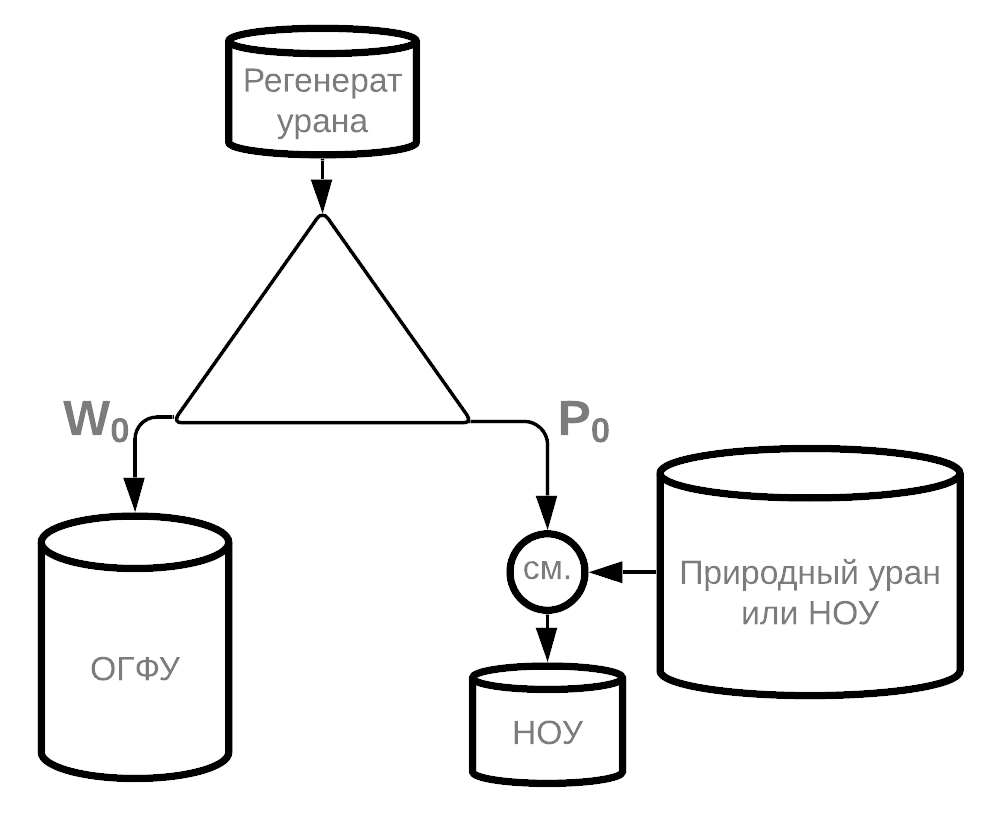
\includegraphics[scale=0.2]{cascades/ordinary/1}}
  \caption{Схема разбавления предварительно обогащенного регенерата природным ураном или низкообогащенным ураном. Обозначения: $P_0$ -- поток отбора легкой фракции каскада; $W_0$ -- поток отвального ОГФУ тяжелого конца каскада; $CM.$ -- узел смешения, на выходе из которого получается конечный продукт $НОУ$ -- низкообогащенный уран}\label{o1}
\end{figure}

\subsection{Анализ схемы с разбавлением предварительно обогащенного регенерата природным ураном}

Рассмотрим каскадную схему, когда регенерат второго рецикла обогащается до уровня, превышающего требуемую концентрацию $^{235}$U, а затем разбавляется природным ураном (рис. \ref{o1}). Такая схема осуществляет снижение накопления четных изотопов в регенерате урана за счет разбавления четных изотопов $^{232,234,236}$U смесью природного урана, не содержащей минорных изотопов $^{232,236}$U, добиваясь требуемого условием задачи содержания изотопа $^{235}$U в финальном продукте-низкообогащенном уране, а также добиваясь выполнения ограничения на  $^{232}$U.

Тогда как получаемая смесь должна одновременно соответствовать требуемой величине обогащения по $^{235}$U, отвечать ограничению по $^{232}$U и удовлетворять условию компенсации $^{236}$U, то есть должны выполняться ограничения на 3 величины, связанные с этими концентрациями. При этом управляющих параметров в такой численной задаче, представляющей из себя систему двух уравнений с невязками $\delta_1$, $\delta_2$ \ref{d1}-\ref{d2} только два:

\begin{enumerate}
  \item выходная концентрация $^{235}$U обогащаемого регенерата;
  \item соотношение смешиваемых потоков $P_0$ и природного урана.
\end{enumerate}

При этом важно отметить, что хоть выходная концентрация $^{235}$U и является управляющим параметром, ее изменение неминуемо влечет за собой изменение и концентраций $^{236}$U и $^{232}$U, тем самым внося дополнительную неопределенность в решение задачи.

Это значит, что нахождение строго удовлетворяющего всем условиям решения не гарантировано и зависит от исходного состава регенерированного урана, а также условий к производимому в схеме НОУ-продукт. Возможность получить такое решение будет проанализирована далее.   

Результаты вычислительных экспериментов, проделанных для состава второго рецикла, показали, что для данного состава не удалось найти решение задачи, которое бы одновременно отвечало требованиям на концентрации изотопов $^{232,234,236}$U в конечном НОУ-продукте. Невозможность нахождения подобного решения иллюстрируют кривые представленные на рис. \ref{fig:deltas_ordinar}.

Они отражают зависимости величин $\delta_1$ и $\delta_2$ \ref{d1}-\ref{d2} от соотношения смешиваемых потоков, взятых для различных значений концентрации $^{235}$U (рис. \ref{fig:deltas_ordinar}) в обогащенном регенерате.

\begin{equation} \label{d1} 
  \delta_1=\left[C_{235}^P-\left(C_n^P+ККР\times C_{236}^P\right)\right], где ККР -- коэффициент компенсации реактивности
  \end{equation} 
  \begin{equation} \label{d2} 
    \delta_2=\left[C_{232}^P-5\times10^{-7}\right]\times10^5.             
\end{equation}

По своему физическому смыслу величина $\delta_1$ представляет собой абсолютное отклонение концентрации изотопа $^{235}$U (выраженное в долях) в окончательном продукте (после смешивания) от требуемой величины, с учетом компенсации $^{236}$U, а величина $\delta_2$ представляет собой разность фактической концентрации $^{232}$U в окончательном продукте и требуемой величины в соответствии с принятым ограничением. А чтобы сопоставить указанные величины на одном рисунке, $\delta_2$ была взята с поправкой (умножена на специально подобранный числовой коэффициент). То есть, величины $\delta_1$ и $\delta_2$ соответствуют невязкам в решении системы нелинейных уравнений, которые, в случае нахождения решения системы будут равняться нулю (величине, не превышающей максимально допустимую погрешность вычислений, которая в численном методе решения задается с помощью специальной системной переменной).

\begin{figure}[ht]
  \begin{minipage}{.5\textwidth}
    \centering
    % include first image
    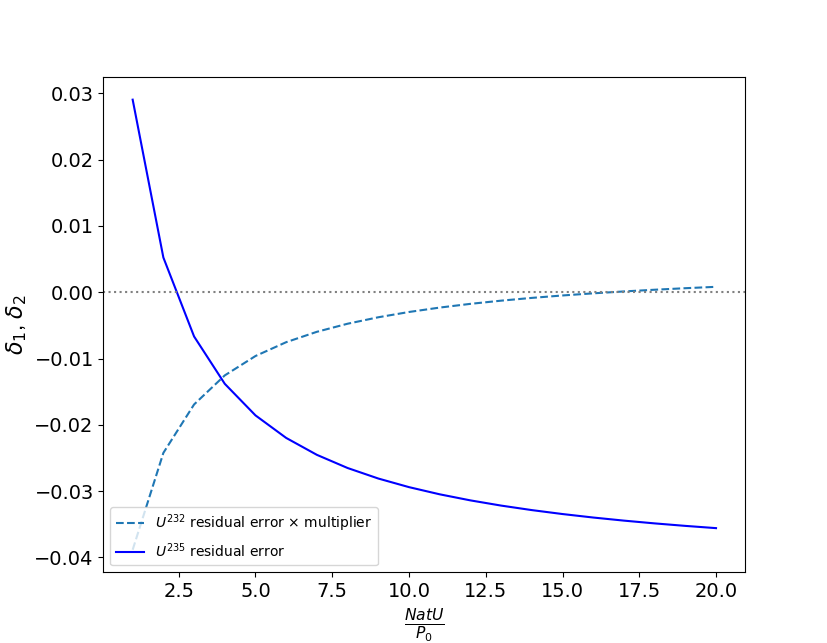
\includegraphics[width=.8\linewidth]{images/plots/15}  
    \caption{Концентрация $^{235}$U в предварительно обогащенном регенерата равна 15\%}
  \end{minipage}
  \begin{minipage}{.5\textwidth}
    \centering
    % include second image
    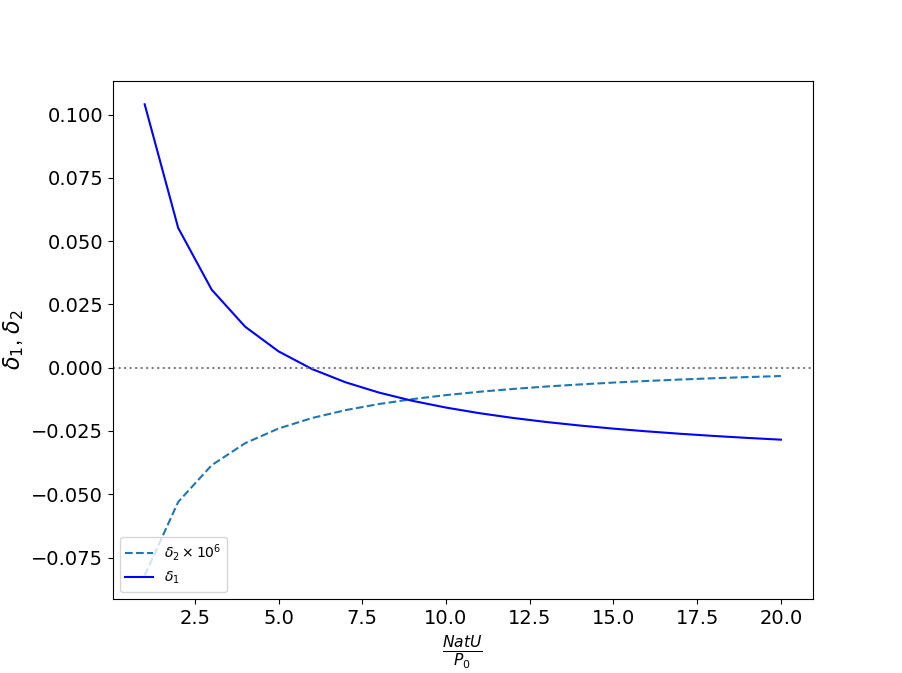
\includegraphics[width=.8\linewidth]{images/plots/30}  
    \caption{Концентрация $^{235}$U в предварительно обогащенном регенерата равна 30\%}
  \end{minipage}
  \begin{minipage}{.5\textwidth}
    \centering
    % include second image
    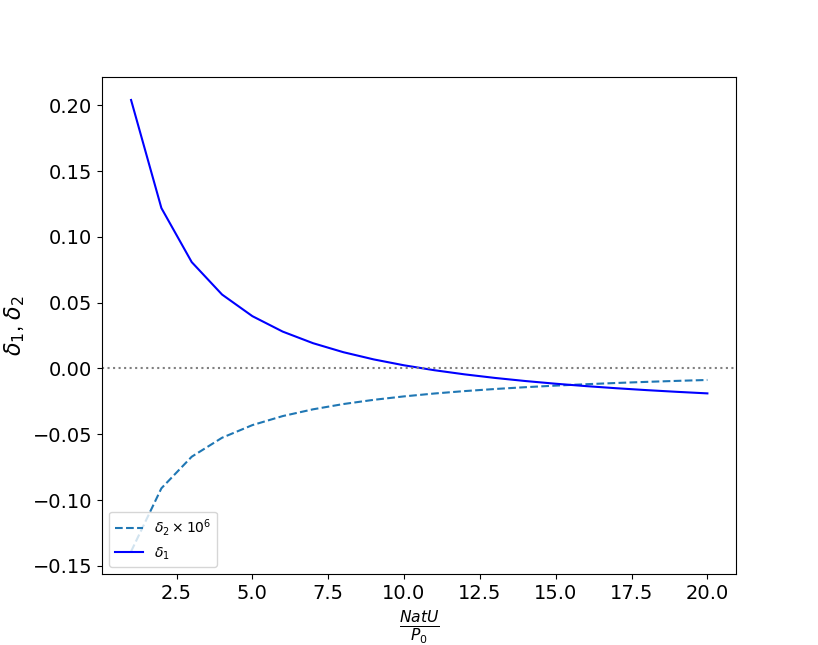
\includegraphics[width=.8\linewidth]{images/plots/50}  
    \caption{Концентрация $^{235}$U в предварительно обогащенном регенерата равна 50\%}
  \end{minipage}
  \begin{minipage}{.5\textwidth}
    \centering
    % include second image
    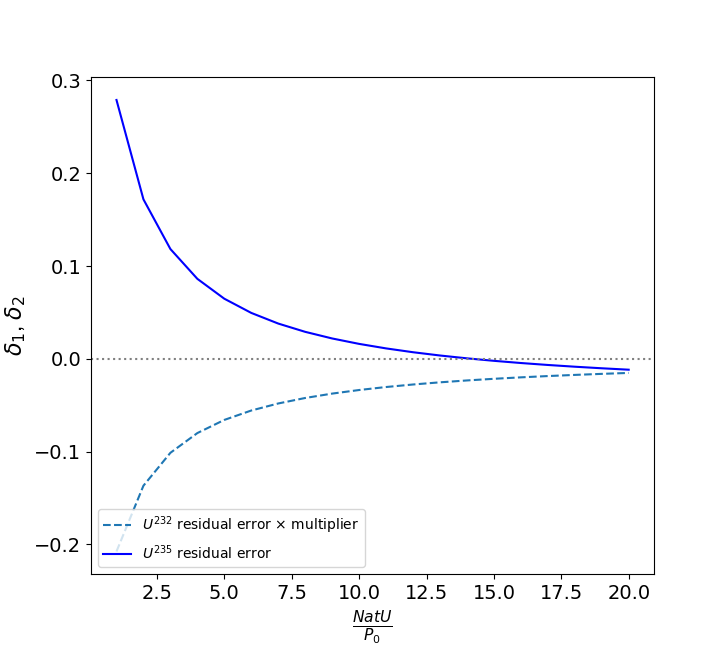
\includegraphics[width=.8\linewidth]{images/plots/65}  
    \caption{Концентрация $^{235}$U в предварительно обогащенном регенерата равна 65\%}
  \end{minipage}
  \caption{Невязки для $^{235}$U и $^{232}$U. Обозначения: $\frac{NatU}{P_{0}}$ -- отношение доли природного урана к потоку обогащенного регенерата.}
  \label{fig:deltas_ordinar}
 \end{figure}

Итак, для успешного решения СНАУ, определяемой системой двух нелинейных уравнений с невязками $\delta_1$ и $\delta_2$ \ref{d1}-\ref{d2}, обе эти величины должны равняться нулю для одного и того же значения аргумента, чего не удается достичь на приведенных рисунках.

Таким образом, полученные результаты показывают невозможность применения каскадной схемы с разбавлением обогащенного регенерата природным (рис. \ref{o1}), когда будут одновременно выполнены условия на $^{235}$U и $^{232}$U, для решения задачи в выбранной постановке. Иными словами, невозможно наладить процесс обогащения регенерата для возврата его в ядерный топливный цикл в условиях многократного рецикла на базе схемы, основанной на идее разбавления предварительно обогащенного регенерата изотопной смесью природного урана.

\subsection{Анализ схемы с разбавлением предварительно обогащенного регенерата низкообогаченным ураном (НОУ) на основе природного урана}

Рассмотрим замену в схеме с предварительно обогащенным регенератом (рис. \ref{o1}) разбавителя -- природного урана -- на низкообогащенный уран, не содержащий минорных изотопов (например, изготовленный из природного урана). В этом случае имеется решение, когда одновременно выполнены условия равенства нулю обеих невязок. Этот факт обусловлен появлением в таком варианте схемы дополнительного управляющего параметра -- концентрации $^{235}$U в потоке разбавителя $НОУ$.

Чтобы исследовать рабочую область параметров для данной схемы, а также определить при каких параметрах схема наиболее эффективна, исследуются диапазоны следующих параметров схемы: $^{235}$U в концах каскада: $P_0$ и $W_0$ (рис. \ref{o1}). Это поможет проиллюстрировать как меняются доли природного урана и регенерата в конечном продукте и как ведет себя работа разделения.

\begin{figure}[ht]
  \centerfloat{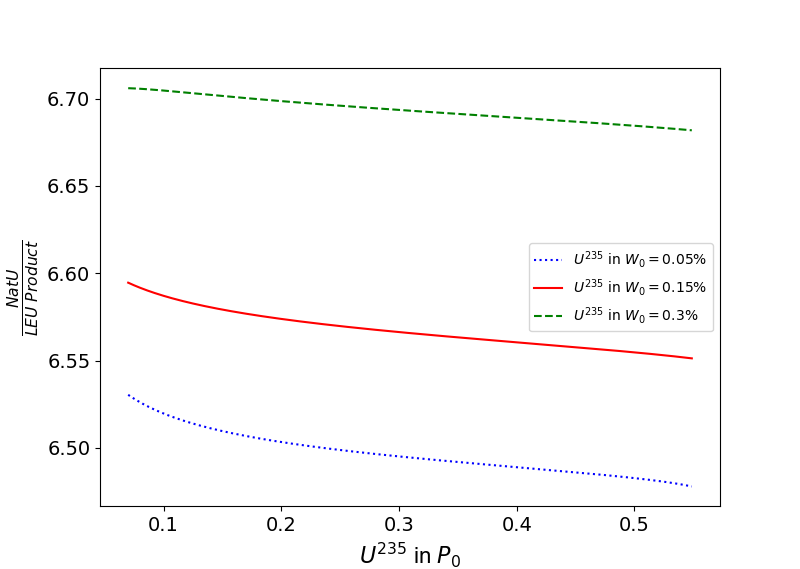
\includegraphics[scale=0.5]{images/plots/sc2_2}}
  \caption{Расход природного урана на единицу НОУ-продукта  для различных концентраций $^{235}$U в потоках продукта и отвала каскада, обогащающего регенерат}\label{fig:sc2_2}
\end{figure}

Рис. \ref{fig:sc2_2} иллюстрирует зависимость расхода природного урана (NatU) на единицу НОУ-продукта (LEU Product) от концентрации $^{235}$U в обогащенном регенерате ($P_0$ на рис. \ref{o1}) для разных значений концентрации $^{235}$U в отвале каскада, получаемом из регенерата. Значения уровня расхода природного урана на уровне $\approx$6,5--6,7 для всего исследуемого диапазона параметров, близки к расходу природного урана в схеме ординарного каскада, когда он используется без добавки из регенерата для производства свежего НОУ топлива, аналогичного по исходным требованиям к продукту. Для значений концентрации $^{235}$U в $W_0$ на уровнях 0,05\% и 0,15\%, значения расхода природного урана в схеме ординарного каскада для обогащения природного урана, будут составлять $\approx$7,41 и $\approx$8,55, соответственно. Таким образом, при заданном интервале параметров, использование схемы с разбавлением обогащенного регенерата позволяет обеспечить экономию природного урана на уровне 15\%--28\%.

Заметим, что по $^{235}$U регенерат обогащается до значений (рис.  \ref{fig:sc2_2}), превышающих пороговое значение для НОУ в 20\%, что может быть неприемлемым в виду требований соблюдения условий нераспространения ядерных материалов \cite{brownOriginsSignificanceLimit2016}. Именно эти значения соответствуют наилучшим показателям экономии природного урана, хотя переход 20\%-й границы для $^{235}$U, дает прирост экономии природного урана менее 1\%. Более существенное улучшение экономии (>3\%), как видно на графике \ref{fig:sc2_2}, происходит с ростом уровня извлечения $^{235}$U из регенерата при понижении концентрации $^{235}$U в обедняемом потоке регенерата $W_0$. Эффект экономии природного урана от понижения $^{235}$U в $W_0$, а также от повышения $^{235}$U в $P_0$, обсуловлен возможностью использовать НОУ-разбавитель с более низким уровнем $^{235}$U, что проиллюстрировано на рис.\ref{fig:sc2_LEU_D}.

Уменьшение концентрации $^{235}$U в обедняемом потоке регенерата $W_0$ связано с еще одним преимуществом: более высокий уровень обеднения исходной смеси ($^{235}$U в $W_0$ при концентрации 0,05\%), дает существенный вклад в экономию работы разделения, что показано на рис.\ref{Figure_13}, за счет более эффективного извлечения $^{235}$U из регенерата, в котором исходно больше доля этого изотопа, чем в природном уране, из которого нарабатывается НОУ-разбавитель, подмешиваемый к $P_0$. Область отрицательных значений потерь работы разделения (SW loss) на рис. \ref{Figure_13} соответствует величине экономии работы разделения, относительно ординарного каскада, взятой с обратным знаком. Слияние кривых, соответствующих различным концентрациям $^{235}$U в обогащенном регенерате, обусловлено эквивалентностью масс $^{235}$U в каждом из этих потоков, что отражает постоянство вклада обогащенного регенерата в формирование конечного продукта.

\begin{figure}[ht]
  \centerfloat{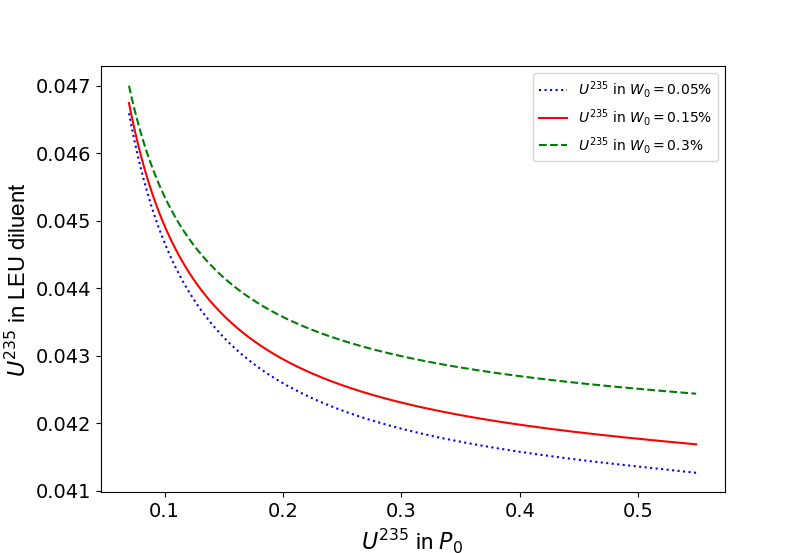
\includegraphics[scale=0.5]{images/plots/sc2_LEU_D}}
  \caption{Концентрация $^{235}$U в разбавителе, необходимая для получения свежего НОУ для различных концентраций $^{235}$U в потоках продукта и отвала каскада, обогащающего регенерат}\label{fig:sc2_LEU_D}
\end{figure}

\begin{figure}[ht]
  \centerfloat{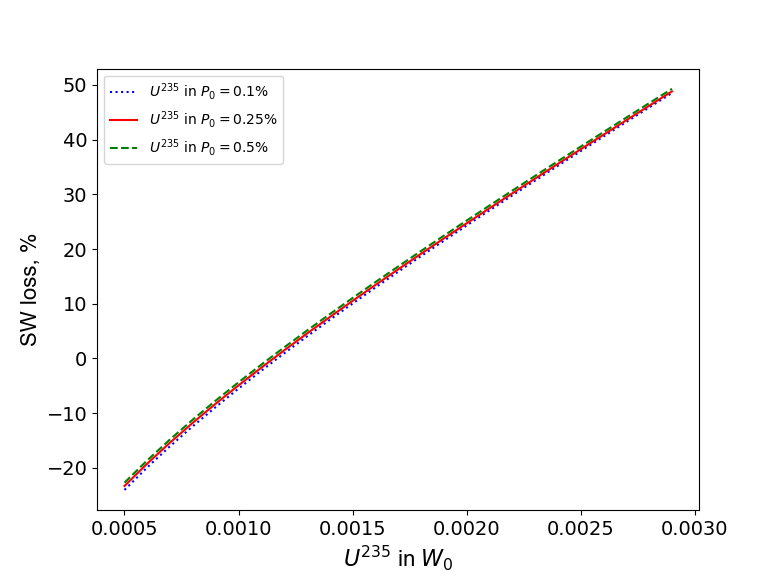
\includegraphics[scale=0.5]{images/plots/Figure_13}}
  \caption{Потери работы разделения по отношению к ординарному каскаду для обогащения природного урана для различных концентраций $^{235}$U в потоках продукта и отвала каскада, обогащающего регенерат}\label{Figure_13}
\end{figure}

Анализ графика \ref{Figure_10} зависимости расхода регенерата на единицу НОУ-продукта ($\frac{NatU}{P_{0}}$) от концентрации $^{235}$U в $W_0$, показывает невозможность выполнить условия возврата заданной доли регенерата на единицу продукта при любых параметрах каскадной схемы ($^{235}$U в $W_0$ и в $P_0$). Причем пропорция используемого регенерата к НОУ-продукту меняется лишь незначительно концентрацией $^{235}$U в $W_0$, а удлинение обогащающей части каскада (рост $^{235}$U в $P_0$) не приводит росту вовлечения регенерата.

\begin{figure}[ht]
  \centerfloat{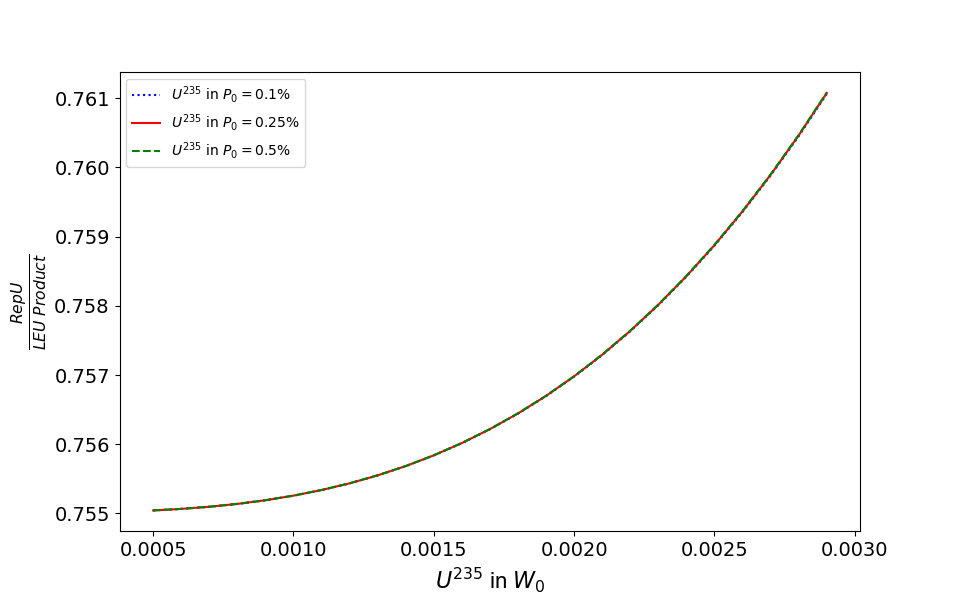
\includegraphics[scale=0.5]{images/plots/Figure_10}}
  \caption{Расход регенерата на единицу конечного НОУ-продукта для различных концентраций $^{235}$U в потоках продукта и отвала каскада, обогащающего регенерат}\label{Figure_10}
\end{figure}

% Проиллюстрировать затраты на работу разделения от составных  частей каскадной схемы, можно с помощью рис.\ref{myplot}, который показывает, что доля центрифуг для приготовления разбавителя из природного урана выше, чем доля центрифуг, задействованных для предварительного обогащения регенерата, и эта пропорция уменьшается с понижением содержания $^{235}$U в $W_0$.

% \begin{figure}[ht]
%   \centerfloat{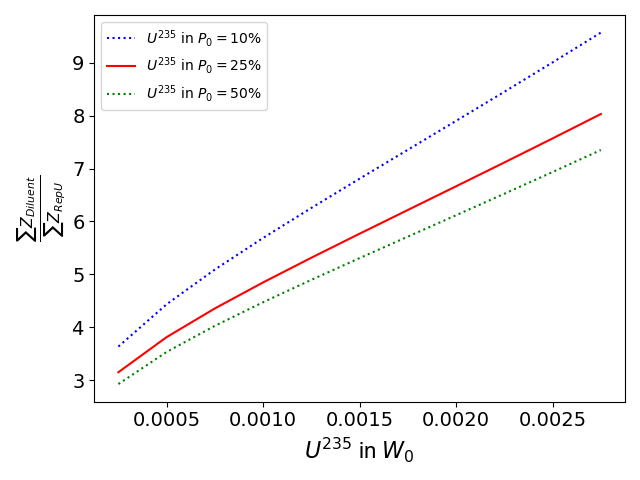
\includegraphics[scale=0.5]{images/plots/myplot}}
%   \caption{Отношение количества центрифуг в каскаде, производящем разбавитель из природного урана, к количеству центрифуг, задействованных для предварительного обогащения регенерата, для различных концентраций $^{235}$U в потоках продукта и отвала каскада, обогащающего регенерат}\label{myplot}
% \end{figure}

В качестве вывода, который можно заключить на основе анализа рис.\ref{fig:sc2_2}-\ref{Figure_10}, схема с разбавлением обогащенного регенерата смесью, не содержащей минорных изотопов, непригодна для решения поставленной задачи обогащения в условиях многократного рецикла. Анализ рабочих диапазонов для схемы демонстрирует, что уменьшение концентрации $^{235}$U в $W_0$ позволяет достичь экономии природного урана на единицу продукта (рис. \ref{fig:sc2_2}), за счет понижения концентрации $^{235}$U в НОУ-разбавителе (рис. \ref{fig:sc2_LEU_D}), а также сэкономить работу разделения (рис. \ref{Figure_13}), при том что расход регенерата на единицу продукта будет меньше на пренебрежимо малую величину (рис. \ref{Figure_10}). Анализ графиков (рис.\ref{fig:sc2_2} и \ref{fig:sc2_LEU_D}) демонстрирует возможность с увеличением уровня обогащения регенерата получить рост экономии природного урана за счет меньшей необходимой концентрации $^{235}$U в НОУ-разбавителе. Однако, следует отметить, что превышение концентрации $^{235}$U уровня НОУ в 20\% может быть недопустимо на некоторых разделительных производствах, так как такой материал попадает в категорию высокообогащенного урана (ВОУ), на производство которого наложены ограничения \cite{gusevProliferationResistanceAnalysis2019}.


\subsection{Анализ схемы с разбавлением предварительно обогащенного регенерата природным ураном}

Перейдем к анализу схемы с разбавлением предварительно обогащенного природного урана регенератом, изображенной на рис. \ref{o2}. Принцип такой схемы состоит в том, что предварительно обогащенный природный уран смешивается с возвращаемым в топливный цикл регенерированным ураном. Степень предварительного обогащения (перед смешением) природного урана и пропорция смешения обогащенного потока с регенератом определяются изходя из условий задачи на содержание в конечном продукте $^{235}$U, поправки на компенсацию $^{236}$U, а также ограничение присутствия $^{232}$U. Таким образом, в такой схеме, как и в схеме с разбавлением предварительно обогащенного регенерата природным ураном (рис. \ref{o1}), на одну независимую переменную (степень свободы) меньше, чем условий в задаче, поскольку мы не можем контролировать разбавитель до его смешивания с обогащенной в каскаде смесью. Проанализируем возможность нахождения решения поставленной задачи с помощью этой схемы.


\begin{figure}[ht]
  \centerfloat{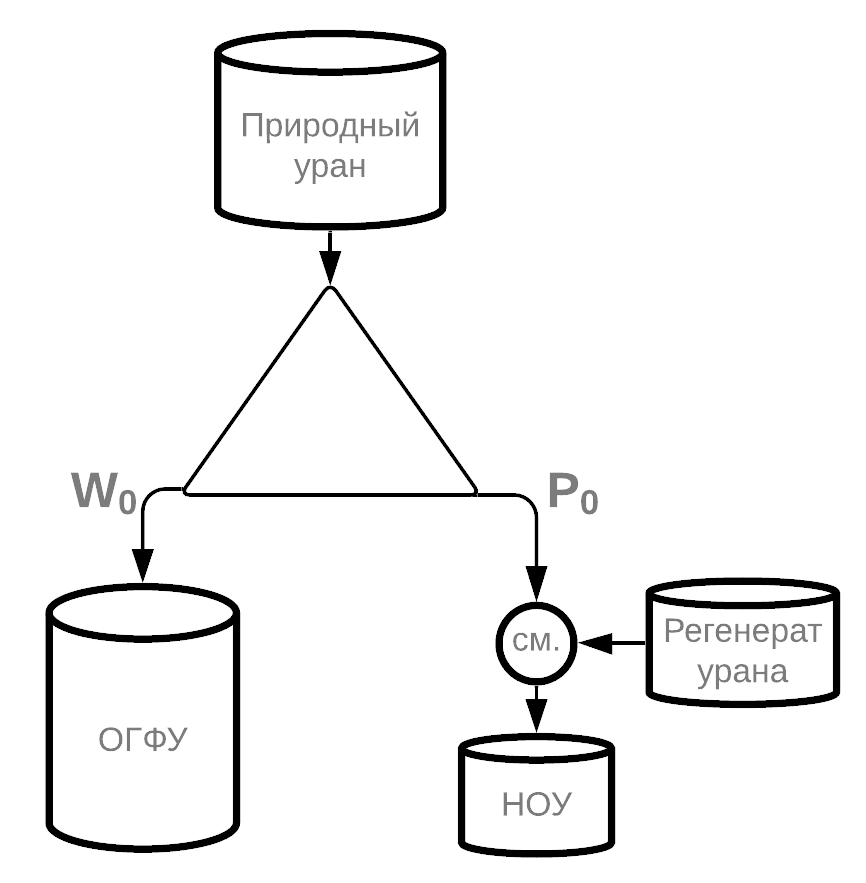
\includegraphics[scale=0.2]{cascades/ordinary/2}}
  \caption{Схема каскада с разбавлением предварительно обогащенного природного урана регенератом. Обозначения: $P_0$ -- поток отбора легкой фракции каскада; $W_0$ -- поток отвального ОГФУ тяжелого конца каскада; $CM.$ -- узел смешения, на выходе из которого получается конечный НОУ-продукт $НОУ$  -- низкообогащенный уран}\label{o2}
\end{figure}

Из результатов вычислительных экспериментов, проведенных для входного состава регенерата второго рецикла, следует, что для рассматриваемой схемы с разбавлением предварительно обогащенного природного урана регенератом, принимая жесткие требования к четным изотопам, возможно получение единственного решения. Однако, как и в случае применения схемы рис. \ref{o1}, не удается добиться условия возврата заданной пропорции регенерата, так как в найденном решении недостаточен расход регенерата на единицу НОУ-продукта и составляет ($\approx$0,75). При этом уровень обогащения природного урана в каскаде достигает $\approx$16\% при различных значениях концентрации $^{235}$U в отвале этого каскада. Следовательно, как показано на примере изотопного состава регенерированного урана второго рецикла, такая схема возврата урана в цикл, созданная на основе ординарного трехпоточного каскада, не адекватна поставленной задаче многократного рецикла.

\subsection{Анализ схемы с разбавлением регенерата природным ураном перед подачей в ординарный трехпоточный каскад}

Еще одним вариантом реализации простейшей модификации ординарного каскада, используемого для обогащения природного урана, является предварительное смешение природного урана с регенератом перед подачей результирующей смеси на питание каскада. Такая схема изображена на рис. \ref{o3}. Суть ее работы состоит в том, что пропорция смешения сырьевых природного и регенерированного урана  определяется предварительно исходя из ограничений на четные изотопы в конечном НОУ-продукте.

\begin{figure}[ht]
  \centerfloat{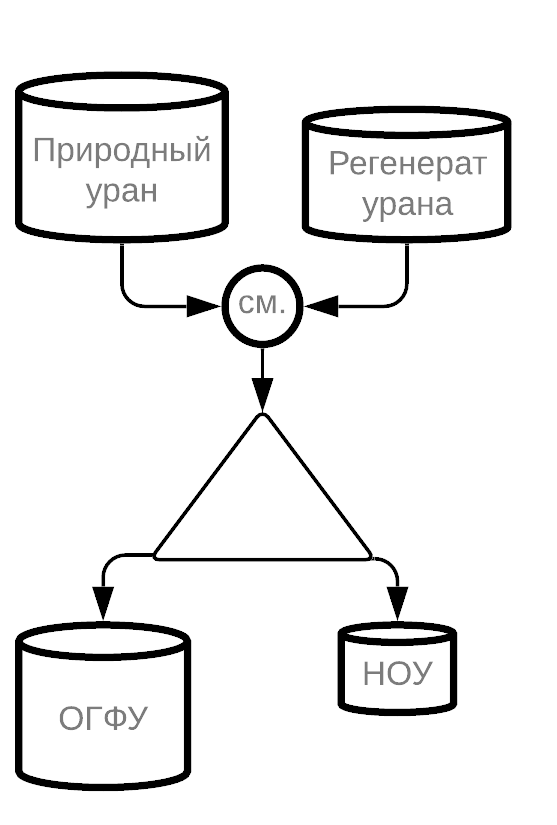
\includegraphics[scale=0.25]{cascades/ordinary/3}}
  \caption{Схема каскада со смешением регенерата и природного урана перед подачей на питание ординарного каскада. Обозначения: $P_0$ -- поток отбора легкой фракции каскада; $W_0$ -- поток отвального ОГФУ тяжелого конца каскада; $CM.$ -- узел смешения входящих сырьевых потоков; $НОУ$ -- конечный НОУ-продукт схемы}\label{o3}
\end{figure}

Как показывает анализ поиска решений схемы с разбавлением регенерата природным ураном перед подачей на питание каскада (рис. \ref{o3}), при использовании состава регенерата второго рецикла, в этом каскаде также невозможно достижение требуемой пропорции расхода регенерата урана на единицу финального продукта (рис. \ref{sc3_1.second}). Для каждого рассматриваемого значения концентрации $^{235}$U в $W_0$, имеется единственно возможное решение системы двух нелинейных уравнений, где обе невязки $\delta_1$ и $\delta_2$  обращаются в нуль, и в этих решениях, расход регенерата на единицу продукта ($\frac{RepU}{LEU Produce}$) не превышает 80\%. Эти решения изображены на пересечения кривых (рис. \ref{sc3_1.second}) с вертикальными и горизонтальными прямыми для указания на принимаемые ими значения расхода регенерата на единицу продукта ($\frac{RepU}{LEU Produce}$), а также доли регенерированного урана в смеси, питающей каскад ("RepU fraction in feed" на верхней горизонтальной оси).


\begin{figure}[ht]
  \centerfloat{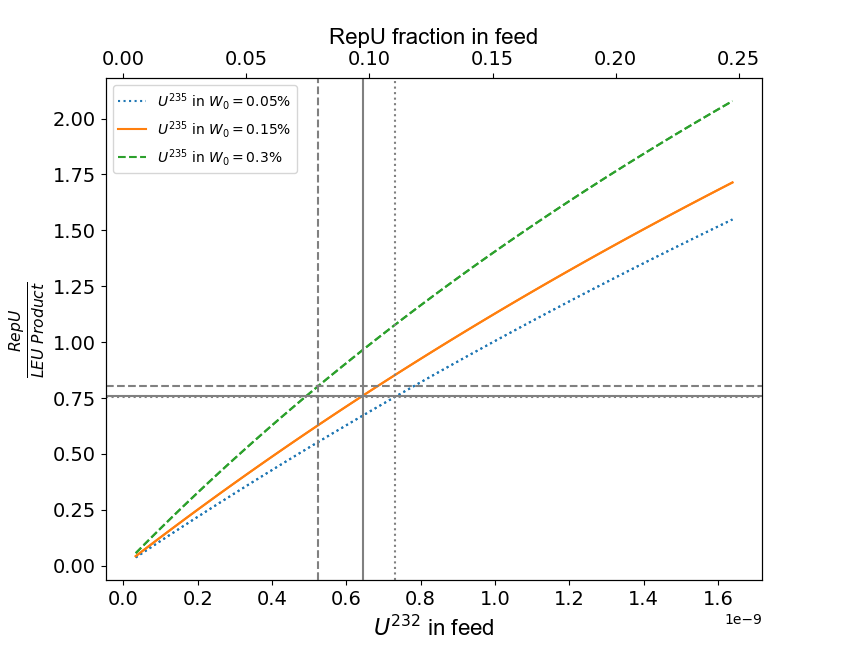
\includegraphics[scale=0.5]{images/plots/sc3_1.second}}
  \caption{Расход регенерированного урана на единицу НОУ-продукта  при различной концентрации $^{232}$U в питающем потоке каскада для различных концентраций $^{235}$U в потоке отвала}\label{sc3_1.second}
\end{figure}

% Рис.\ref{sc3_2.second} показывает расход природного урана на единицу продукта для того же набора найденных решений.

% \begin{figure}[ht]
%   \centerfloat{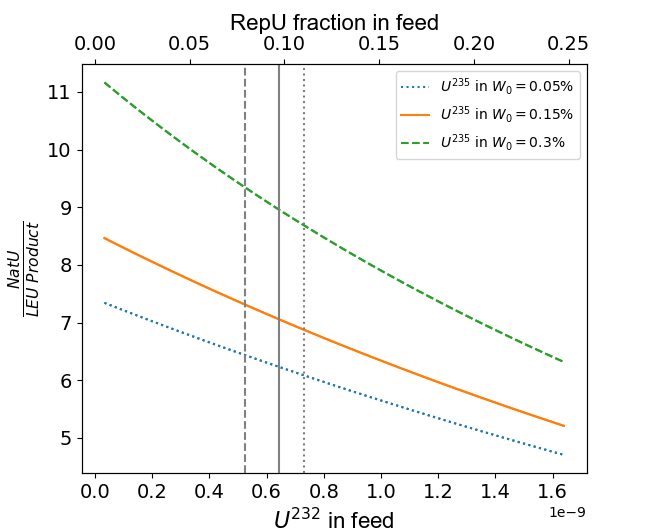
\includegraphics[scale=0.5]{images/plots/sc3_2.second}}
%   \caption{Расход природного урана на единицу НОУ-продукта  при различной концентрации $^{232}$U в питающем потоке каскада для различных концентраций $^{235}$U в потоке отвала}\label{sc3_2.second}
% \end{figure}


\subsection{Общий вывод для схем возврата регенерата в ЯТЦ на основе ординарного каскада}

Таким образом, численные эксперименты доказали, что использование каскадов, являющихся простейшими модификациями ординарного трехпоточного каскада, не удовлетворяет условиям многократного рецикла урана.

При этом закономерно возникает следующих вопрос: возможно ли априорно оценить способность рассматриваемой схемы решить поставленную задачу? Для ответа на этот вопрос приведены следующие оценки.

Согласно уравнениям балансов материальных потоков \ref{GrindEQ__1_21_}, из которых получен частный случай путем предельного перехода для самого легкого изотопа в ряду \ref{eq_232_balance}, для схем на основе единственного ординарного каскада, достижение требуемого соотношения  облученного топлива к свежему -- задействование складских запасов регенерата в количестве эквивалентом произоводимому НОУ-продукту, то есть 1:1 -- а значит соответствующего $\approx$0,93 долям затрачиваемого регенерата на единицу НОУ-продукта, может быть обеспечено только тогда, когда концентрация $^{232}$U в исходном регенерате ниже, чем ограничение на присутствие $^{232}$U в конечном продукте. Это соответствует уравнению \ref{eq_232_balance}:

\begin{equation}
\label{eq_232_balance}
  C_{232_{U}}^{P} \approx \frac{F}{P} C_{232_{U}}^{F}
\end{equation}

С помощью уравнения \ref{eq_232_balance} можно вычислить максимально возможную долю питающего потока, содержащего $^{232}$U, как неизвестную переменную уравнения \ref{eq_232_balance}. При этом предполагая, что весь исходный $^{232}$U окажется в конечном счете в продукте, так как его относительный коэффициент обогащения является самым высоким в ряду изотопов в виду того, что $^{232}$U является самым легким изотопом. На основе состава регенерата второго рецикла получаем \ref{eq_232_balance_X}:

\begin{equation}
  \label{eq_232_balance_X}
    5 \times 10^{-7} \% \approx X \times 6.622 \times 10^{-7} \% \Rightarrow X \approx 0.755
\end{equation}

Но, так как $\frac{F}{P} = X$ требуется на уровне $\approx$0,93 для достижения условия, накладываемого учетом за оборотом ядерных материалов, можно сделать вывод, что полностью вернуть регенерат в топливный цикл с помощью схем простейшей модификации ординарного каскада невозможно.

В качестве следующей аналитической оценки, вычислим предельный вклад $^{235}$U от используемого регенерата. На этот раз необходимо учитывать концентрацию $^{235}$U и в потоке отвала (ОГФУ), так как значительное количество этого изотопа попадает в отвал каскада. Из балансных уравнений \ref{GrindEQ__1_21_} на основе данных концентрации $^{235}$U в составе регенерата второго рецикла, а также полученной выше достижимой пропорции  $\frac{F}{P} = \approx 0.755$, получаем:

\begin{equation}
  \label{eq_235_balance_X}
   \frac{P*C_{235}^{P} - F_{регенерат}*C_{235}^{F_{регенерат}}}{P*C_{235}^{P}} \approx 0.0078
\end{equation}

Отсюда, сравнивая полученное значение с требуемой концентрацией $^{235}$U, можно вычислить предельный вклад $^{235}$U от регенерата, который будет составлять $\approx$16\% ($0.0078/0.0495\approx0.16$), что соответствует экономии природного урана. В реальной задаче, к сожалению, эта величина экономии будет еще меньше из-за необходимости компенсации по $^{236}$U.

В результате, поскольку количество $^{232}$U в исходном регенерате второго цикла превышает ограничение в $5\cdot10^{-7}$\%, невозможно обеспечить возврат регенерированного урана в ЯТЦ в условиях многократного рецикла с помощью простейших модификаций ординарного каскада, где, либо регенерированный уран предварительно обогащается, либо используется как разбавитель предварительно обогащенного природного урана.

Таким образом, анализ схем на основе базового трехпоточного каскада демонстрирует потребность в модификации компоновок разделительного оборудования в контексте многократного рецикла урана, что и составляет цель диссертационной работы.


\section{Обоснование необходимости составных схем}\label{sec:ch2/sec2}

Как следует из вышеприведенных расчетов, на текущий момент имеются способы, позволяющие принципиально решить проблему выполнения требования по четным изотопам урана при обогащении регенерата, и основной проблемой, решаемой в рамках настоящей диссертационной работы, является поиск варианта каскадной схемы, позволяющей одновременно выполнить условия по четным изотопам и задействовать в обогащении весь имеющийся регенерат, что важно, как было сказано ранее, для того, чтобы избежать накопления регенерированного урана, хранение которого требует затрат.

Если анализировать причины невозможности возврата регенерата в производство топлива в многочисленных модификациях каскада для обогащения многократно облученного регенерата, то становится очевидным, что это, во многом, связано с нарастанием относительных концентраций “легких” изотопов (в первую очередь $^{232}$U) и
$^{235}$U, а поскольку данные изотопы концентрируются вместе на “легком” конце каскада, то единственным способом понизить отношение их концентраций -- это разбавить материалом, не содержащим $^{232}$U, например на входе в каскад. А, как показали сделанные в этой главе вычислительные эксперименты, для составов с достаточно высоким исходным содержанием $^{232}$U невозможно подобрать разбавитель такой, чтобы удовлетворить одновременно и условие полного возврата регенерата в цикл и условия на содержание четных изотопов.

Из приведенного выше анализа вытекает необходимость использовать каскады, предназначенные для отделения друг от друга изотопов легкой фракции: $^{232,233,234}$U и более тяжелой: $^{235,236,238}$U. Такие схемы основаны на двух связанных каскадах, где в первом каскаде изотоп $^{235}$U обогащается с одновременным увеличением концентрации изотопов $^{232}$U и $^{234}$U, а во втором каскаде смесь изотопов разделяется на легкую ($^{232,233,234}$U) и тяжелую фракции ($^{235,238}$U) (рис. \ref{fig:double_ru}) \cite{smirnovApplyingEnrichmentCapacities2018}.

Дальнейшая работа предполагает с использованием вычислительного эксперимента проведение анализа закономерностей массопереноса в каскадах, которые могут быть использованы для обогащения регенерированного урана в рамках многократного рецикла, для выработки рекомендаций к их применению.

% Из вышеприведенного обоснования невозможности решения задачи полного возврата регенерата в топливный цикл легководных реакторов в условиях многократного рецикла и вытекает необходимость использовать составные каскадные схемы ввиду необходимости  <<пространственного>> разделения легкой изотопной фракции с $^{232}$U, $^{234}$U от с $^{235}$U. Так двойная схема позволяет отделить минорные легкие изотопы $^{232}$U, $^{234}$U в независимом потоке отборной части каскада.
% Так, например, схема (рис. \ref{fig:double_ru}) позволяет во втором каскаде разделить потоки, выделив $^{235}$U в тяжелой фракции, направив $^{232}$U и $^{234}$U в легкую.
% С появлением свойств такого рода у каскадов, вместо привычной дихотомии, выделяющей схемы с приставкой <<много->> (многопоточные схемы, многокаскадные конфигурации), предлагается классифицировать каскады, используемые для обогащения регенерата, как разбавляющие или очищающие, потому что условная граница <<каскад-разбавитель>> -- <<каскад-очиститель>> гораздо лучше подчеркивает сущностные характеристики анализируемых схем, предназначенных для повторного обогащения урана. Так, схема двойного каскада является очищающей, в отличие от схем, основанных на ординарном каскаде, работающих на принципе разбавления.  

% В обзоре (глава 1) диссертации было показано, что такая схема (рис. \ref{fig:double_ru}) не может обеспечить соблюдение заданной пропорции для возврата.

\clearpage